%!TEX encoding = UTF-8 Unicode
% -*- coding: UTF-8; -*-
% vim: set fenc-utf-8

\chapter{Cas d'utilisations}
\label{s:cas_utilisation}

Ce chapitre présente les différents cas d'utilisation pour l'application VisuaLigue.
La figure \ref{fig:cas_utilisation_diag} résume les acteurs du systèmes et les cas d'utilisations.
La suite du chapitre décrit en détails les cas d'utilisations et s'attarde sur les plus importants.

\begin{figure}[htpb]
    \centering
    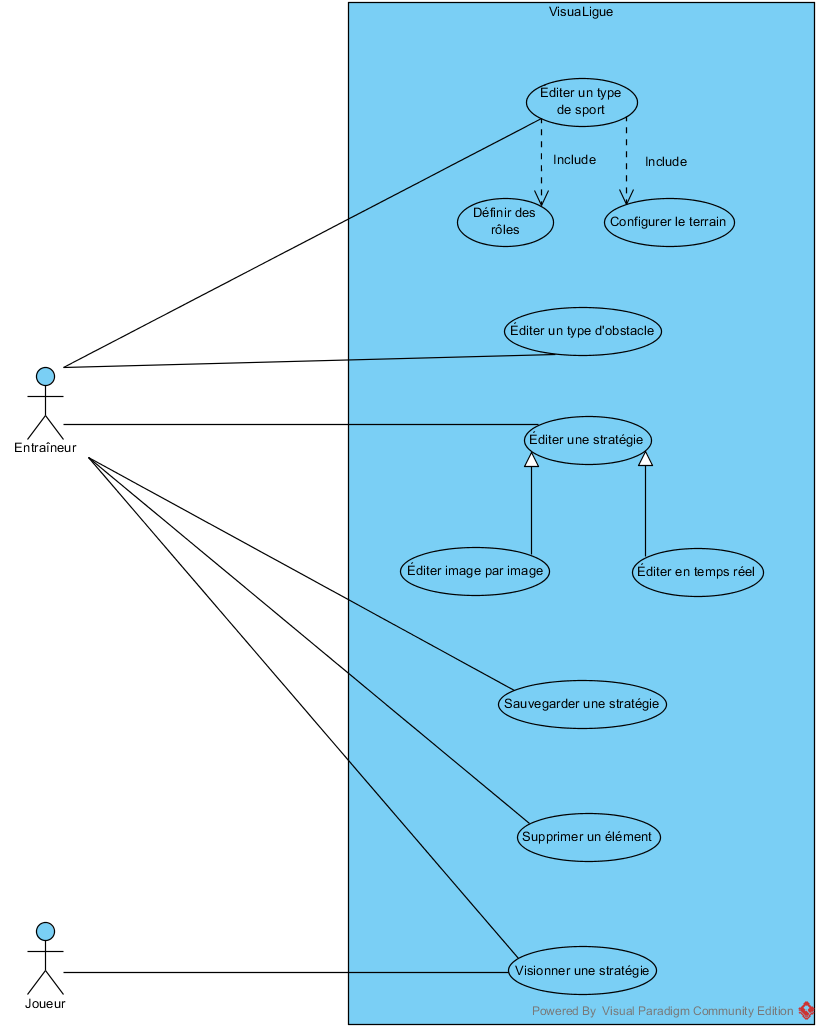
\includegraphics[scale=0.7]{fig/cas_utilisation_diag.png}
    \caption{Diagramme des cas d'utilisations}
    \label{fig:cas_utilisation_diag}
\end{figure}

\newpage



\section{Éditer un type de sport}
\label{sec:ajouter_un_type_de_sport}

\begin{itemize}
    \item \textbf{Cas d'utilisation:} Éditer un type de sport
    \item \textbf{Syst\`eme:} VisuaLigue
    \item \textbf{Acteur principal:} Entra\^ineur
    \item \textbf{Pr\'erequis:} Aucun.
    \item \textbf{Parties prenantes et int\'er\^ets:}
        \begin{itemize}
            \item Entraîneur : Veut pouvoir cr\'eer facilement le type de sport que pratique son équipe ainsi que configurer les paramètres de ce sport.
        \end{itemize}
    \item \textbf{Garanties en cas de succ\`es :} Le sport est ajout\'e \`a la liste des sports existants et peut \^etre utiliser lors de la cr\'eation de strat\'egies.
    \item \textbf{Sc\'enario principal:}
        \begin{enumerate}
            \item L'entra\^ineur cr\'ee un sport, le nomme.
            \item Ensuite il ajoute les r\^oles des joueurs du sport.
            \item Finalement, il d\'efini un terrain en dessinant les lignes et en sp\'ecifiant les dimensions.
        \end{enumerate}
    \item \textbf{Autres situations:}
        \begin{itemize}
            \item \textbf{1a. Sport d\'ej\`a existant:} Si le sport existe d\'ej\`a dans l'application, un message d'avertissement appara\^it pour signaler que le sport existe d\'ej\`a.
                L'entraîneur peut d\'ecider d'effacer ce qui \'etait dans le sport existant, d'enregistrer son sport sous un autre nom, ou d'oublier le sport cr\'e\'e.
            \item \textbf{3a. Ajout d'une image :} L'entraîneur peut ajouter une image plutôt que dessiner les lignes pour représenter le terrain.
        \end{itemize}
    \item \textbf{Fréquence d'utilisation :} Ce cas d'utilisation survient rarement.
\end{itemize}



\section{Définir des rôles}
\label{sec:definir_des_roles}

\begin{itemize}
    \item \textbf{Cas d'utilisation:} D\'efinir des r\^oles
    \item \textbf{Syst\`eme:} VisuaLigue
    \item \textbf{Acteur principal:} Entra\^ineur
    \item \textbf{Parties prenantes et int\'er\^ets:}
        \begin{itemize}
            \item
        \end{itemize}
    \item \textbf{Pr\'erequis :} Aucun.
    \item \textbf{Garanties en cas de succ\`es :}
    \item \textbf{Sc\'enario principal:}
        \begin{enumerate}
            \item L'entraîneur défini une liste de rôles pour un sport.
        \end{enumerate}
    \item \textbf{Autres situations:}
        \begin{itemize}
            \item foo
                \begin{enumerate}
                    \item baz
                \end{enumerate}
        \end{itemize}
    \item \textbf{Fréquence d'utilisation :}
\end{itemize}



\section{Configurer le terrain}
\label{sec:configurer_le_terrain}

\begin{itemize}
    \item \textbf{Cas d'utilisation:} Configurer le terrain
    \item \textbf{Syst\`eme:} VisuaLigue
    \item \textbf{Acteur principal:} Entra\^ineur
    \item \textbf{Pr\'erequis:} Aucun.
    \item \textbf{Parties prenantes et int\'er\^ets:}
        \begin{itemize}
            \item Entraîneur: Veut créer un terrain rapidement et facilement. S'il n'a pas d'images pour le terrain, en tracer un doit être facile.
        \end{itemize}
    \item \textbf{Pr\'erequis:}
    \item \textbf{Garanties en cas de succ\`es:} Le terrain est proportionnel par rapport à ses dimensions réels.
    \item \textbf{Sc\'enario principal:}
        \begin{enumerate}
            \item L'entraîneur importe une image.
            \item Il spécifie les dimensions du terrain.
        \end{enumerate}
    \item \textbf{Autres situations:}
        \begin{itemize}
            \item \textbf{1.a Dessiner le terrain} L'entraîneur peut choisir de dessiner les lignes du terrain.
                \begin{enumerate}
                    \item L'entraîneur choisit de dessiner le terrain.
                    \item Un application de dessin s'ouvre et l'entraîneur trace les lignes du terrain.
                    \item L'entraîneur sauvegarde son tracer et continue le scénario principal à partir de l'étape 2.
                \end{enumerate}

        \end{itemize}
    \item \textbf{Fréquence d'utilisation :} Ce cas d'utilisation sera utilisé à chaque fois que l'on éditeras un nouveau terrain.
\end{itemize}



\section{Éditer un type d'obstacle}
\label{sec:editer_un_type_d_obstacle}

\begin{itemize}
    \item \textbf{Cas d'utilisation:} \'Editer un type d'obstacle
    \item \textbf{Syst\`eme:} VisuaLigue
    \item \textbf{Acteur principal:} Entra\^ineur
    \item \textbf{Parties prenantes et int\'er\^ets:}
        \begin{itemize}
            \item
        \end{itemize}
    \item \textbf{Pr\'erequis :} Aucun.
    \item \textbf{Garanties en cas de succ\`es :}
    \item \textbf{Sc\'enario principal:}
        \begin{enumerate}
            \item L'entraîneur donne un nom à un obstacle.
            \item Il associe une image.
        \end{enumerate}
    \item \textbf{Autres situations:}
        \begin{itemize}
            \item foo
                \begin{enumerate}
                    \item baz
                \end{enumerate}
        \end{itemize}
    \item \textbf{Fréquence d'utilisation :}
\end{itemize}



\section{\'Editer une stratégie}
\label{sec:ajouter_une_strategie}
\begin{itemize}
    \item \textbf{Cas d'utilisation:} \'Editer une strat\'egie
    \item \textbf{Syst\`eme:} VisuaLigue
    \item \textbf{Acteur principal:} Entra\^ineur
    \item \textbf{Parties prenantes et int\'er\^ets:}
        \begin{itemize}
            \item Entraîneur: Veux pouvoir créer une stratégie composée de multiples déplacements de différents joueurs, ainsi que des passes entre ceux-ci, de manière intuitive et rapide.
        \end{itemize}
    \item \textbf{Pr\'erequis:} Aucun.
    \item \textbf{Garanties en cas de succ\`es:} Les modifications peuvent être visualisé par les utilisateurs.
    \item \textbf{Sc\'enario principal:}
        \begin{enumerate}
            \item L'entraîneur sélectionne la stratégie à éditer.
            \item L'entraîneur assigne les r\^oles aux diff\'erents joueurs.
            \item Ensuite, il peut s\'electionner un joueur et tracer un mouvement ou interargir avec le projectile.
            \item Pendant que le joueur est s\'electionn\'e, une simulation en temps r\'eel des mouvements pr\'ec\'edemment d\'efinis s'ex\'ecute.
            \item La simulation recommence du d\'ebut.
            \item L'entraîneur répète les étapes 3 et 5 pour chaque joueur jusqu'à ce que la stratégie soit terminée.
            \item L'entraîneur exécute \textit{sauvergarder une stratégie}~\ref{sec:exporter_une_strategie}.
        \end{enumerate}
    \item \textbf{Autres situations:}
        \begin{itemize}
            \item \textbf{1a. La stratégie n'existe pas:} L'entraîneur peut décider de créer une nouvelle stratégie en sélectionnant nouvelle stratégie.
                Il devra alors donner un nom à celle-ci.
            \item \textbf{3a. Édition en mode image par image:} L'entraîneur édite la strat\'egie image par image...
                \begin{enumerate}
                    \item L'entraîneur place les joueurs sur le terrain.
                    \item L'entraîneur clique sur un boutton de l'application et avance d'une image. Les joueurs deviennent transparents.
                    \item L'entraîneur clique sur un joueur et le glisse vers sa nouvelle position.
                        Le joueur sélectionné n'est plus transparent.
                    \item L'entraîneur répète l'étape 3 pour tous les joueurs qu'il veut déplacer.
                    \item L'entraîneur répète les étapes 2 à 4 jusqu'à ce qu'il ait terminé sa stratégie.
                    \item L'entraîneur continue le scénario principal à partir de l'étape 6.
                \end{enumerate}
            \item \textbf{*a. visualiser la stratégie}
                À tout moment de l'édition de la stratégie, l'entraîneur peut exécuter \textit{visualiser la stratégie}~\ref{sec:visualiser_une_strategie}.

        \end{itemize}
    \item \textbf{Fr\'equence d'utilisation:}
        Ce cas d'utilisation survient fréquemment.
\end{itemize}



\section{Sauvegarder une stratégie}
\label{sec:exporter_une_strategie}
\begin{itemize}
    \item \textbf{Cas d'utilisation:} Sauvegarder une strat\'egie
    \item \textbf{Syst\`eme:} VisuaLigue
    \item \textbf{Acteur principal:} Entra\^ineur
    \item \textbf{Parties prenantes et int\'er\^ets:}
        \begin{itemize}
            \item
        \end{itemize}
    \item \textbf{Pr\'erequis :} Aucun.
    \item \textbf{Garanties en cas de succ\`es :}
    \item \textbf{Sc\'enario principal:}
        \begin{enumerate}
            \item L'entra\^ineur a modifié une strat\'egie et la sauvegarde.
            \item L'application enregistre les \'el\'ements de la strat\'egie.
        \end{enumerate}
    \item \textbf{Autres situations:}
        \begin{itemize}
            \item \textbf{Exportation dans un format d'image:}
                \begin{enumerate}
                    \item L'entra\^ineur souhaite plut\^ot exporter la strat\'egie dans un format de fichier.
                    \item Il s\'electionne le format de fichier et le nom pour l'exportation.
                    \item L'application convertie la strat\'egie en une image et l'enregistre dans un fichier avec le bon nom.
                \end{enumerate}
        \end{itemize}
    \item \textbf{Fréquence d'utilisation :}
\end{itemize}



\section{Supprimer un \'el\'ement}
\label{sec:supprimer_un_'el'ement}

\begin{itemize}
    \item \textbf{Cas d'utilisation:} Supprimer un \'el\'ement
    \item \textbf{Syst\`eme:} VisuaLigue
    \item \textbf{Acteur principal:} Entra\^ineur
    \item \textbf{Parties prenantes et int\'er\^ets:}
        \begin{itemize}
            \item
        \end{itemize}
    \item \textbf{Pr\'erequis :} Aucun.
    \item \textbf{Garanties en cas de succ\`es :}
    \item \textbf{Sc\'enario principal:}
        \begin{enumerate}
            \item foo
        \end{enumerate}
    \item \textbf{Autres situations:}
        \begin{itemize}
            \item erreur 1
                \begin{enumerate}
                    \item baz
                \end{enumerate}
        \end{itemize}
    \item \textbf{Fréquence d'utilisation :}
\end{itemize}



\section{Visualiser une stratégie}
\label{sec:visualiser_une_strategie}
\begin{itemize}
    \item \textbf{Cas d'utilisation:} Visualiser une strat\'egie
    \item \textbf{Syst\`eme:} VisuaLigue
    \item \textbf{Acteur principal:} Entra\^ineur ou joueur
    \item \textbf{Parties prenantes et int\'er\^ets:}
        \begin{itemize}
            \item L'entra\^ineur: Veux pouvoir visualiser une strat\'egie pour d\'eterminer si elle est ad\'equate.
                Veut pouvoir interrompre la visualisation \`a tout moment pour fournir des explications suppl\'ementaires.
                Veut pouvoir reculer d'un temps fixe la visualisation pour montrer \`a nouveau un segment de la strat\'egie.
                Veut pouvoir red\'ebuter la visualisation pour regarder \`a nouveau la strat\'egie.
            \item Joueur: Veut pouvoir visualiser la strat\'egie pour l'\'etudier.
        \end{itemize}
    \item \textbf{Pr\'erequis:} Il faut que la strat\'egie soit enregistr\'ee dans l'application pour que l'entraîneur puisse la visualiser.
    \item \textbf{Garanties en cas de succ\`es:} \`A la fin de la visualisation la strat\'egie n'a pas \'et\'e modifi\'ee.
    \item \textbf{Sc\'enario principal:}
        \begin{enumerate}
            \item L'utilisateur s\'electionne la strat\'egie \`a visualiser.
            \item Il d\'ebute la visualisation.
            \item La visualisation prend fin lorsque toute la strat\'egie s'est d\'eroul\'ee.
        \end{enumerate}
    \item \textbf{Autres situations:}
        \begin{itemize}
            \item \textbf{1a la strat\'egie est corrompue:}
                \begin{enumerate}
                    \item Lors de la s\'election de la strat\'egie, celle-ci est corrompue.
                    \item Un message d'erreur s'affiche.
                \end{enumerate}
            \item \textbf{2a interrompre la visualisation:}
                \begin{enumerate}
                    \item L'utilisateur \textit{pause} la visualisation.
                    \item L'utilisateur red\'emarre la visualisation.
                    \item On reprend de l'\'etape 2.
                \end{enumerate}
            \item \textbf{2b red\'ebuter la visualisation:}
                \begin{enumerate}
                    \item L'utilisateur \textit{arr\^ete} la visualisation.
                    \item On reprend de l'\'etape 2.
                \end{enumerate}
            \item \textbf{2c reculer d'un temps donn\'ee:}
                \begin{enumerate}
                    \item L'utilisateur \textit{pause} la visualisation.
                    \item Il d\'etermine un temps en secondes.
                    \item Il recule la visualisation.
                    \item Il red\'emarre la visualisation.
                    \item On reprend de l'\'etape 2.
                \end{enumerate}
        \end{itemize}
    \item \textbf{Fréquence d'utilisation :} C'est le cas le plus fr\'equent d'utilisation.
\end{itemize}
